\documentclass[a4paper, 12pt]{article}

\usepackage{arxiv}

\usepackage[T2A]{fontenc}
\usepackage[utf8]{inputenc}
\usepackage[english]{babel}
% \usepackage{cmap}
\usepackage{url}
\usepackage{booktabs}
\usepackage{nicefrac}
\usepackage{microtype}
\usepackage{lipsum}
\usepackage{graphicx}
\usepackage{subfig}
\usepackage[square,sort,comma,numbers]{natbib}
\usepackage{doi}
\usepackage{multicol}
\usepackage{multirow}
\usepackage{tabularx}
\usepackage{authblk}

\usepackage{tikz}
\usetikzlibrary{matrix}

% Algorithms
\usepackage{algpseudocode}
\usepackage{algorithm}

%% Шрифты
\usepackage{euscript} % Шрифт Евклид
\usepackage{mathrsfs} % Красивый матшрифт
\usepackage{extsizes} % Возможность сделать 14-й шрифт

\usepackage{makecell} % diaghead in a table
\usepackage{amsmath,amsfonts,amssymb,amsthm,mathtools,dsfont}
\usepackage{icomma}

\newcommand{\bz}{\mathbf{z}}
\newcommand{\bx}{\mathbf{x}}
\newcommand{\by}{\mathbf{y}}
\newcommand{\bv}{\mathbf{v}}
\newcommand{\bw}{\mathbf{w}}
\newcommand{\ba}{\mathbf{a}}
\newcommand{\bb}{\mathbf{b}}
\newcommand{\bp}{\mathbf{p}}
\newcommand{\bq}{\mathbf{q}}
\newcommand{\bt}{\mathbf{t}}
\newcommand{\bu}{\mathbf{u}}
\newcommand{\bT}{\mathbf{T}}
\newcommand{\bX}{\mathbf{X}}
\newcommand{\bZ}{\mathbf{Z}}
\newcommand{\bS}{\mathbf{S}}
\newcommand{\bH}{\mathbf{H}}
\newcommand{\bW}{\mathbf{W}}
\newcommand{\bY}{\mathbf{Y}}
\newcommand{\bU}{\mathbf{U}}
\newcommand{\bQ}{\mathbf{Q}}
\newcommand{\bP}{\mathbf{P}}
\newcommand{\bA}{\mathbf{A}}
\newcommand{\bB}{\mathbf{B}}
\newcommand{\bC}{\mathbf{C}}
\newcommand{\bE}{\mathbf{E}}
\newcommand{\bF}{\mathbf{F}}
\newcommand{\bomega}{\boldsymbol{\omega}}
\newcommand{\btheta}{\boldsymbol{\theta}}
\newcommand{\bgamma}{\boldsymbol{\gamma}}
\newcommand{\bdelta}{\boldsymbol{\delta}}
\newcommand{\bPsi}{\boldsymbol{\Psi}}
\newcommand{\bpsi}{\boldsymbol{\psi}}
\newcommand{\bxi}{\boldsymbol{\xi}}
\newcommand{\bchi}{\boldsymbol{\chi}}
\newcommand{\bzeta}{\boldsymbol{\zeta}}
\newcommand{\blambda}{\boldsymbol{\lambda}}
\newcommand{\beps}{\boldsymbol{\varepsilon}}
\newcommand{\bZeta}{\boldsymbol{Z}}
% mathcal
\newcommand{\cX}{\mathcal{X}}
\newcommand{\cY}{\mathcal{Y}}
\newcommand{\cW}{\mathcal{W}}

\newcommand{\dH}{\mathds{H}}
\newcommand{\dR}{\mathds{R}}
% transpose
\newcommand{\T}{^{\mathsf{T}}}

% \renewcommand{\shorttitle}{\textit{arXiv} Шаблон}
\renewcommand{\epsilon}{\ensuremath{\varepsilon}}
\renewcommand{\phi}{\ensuremath{\varphi}}
\renewcommand{\kappa}{\ensuremath{\varkappa}}
\renewcommand{\le}{\ensuremath{\leqslant}}
\renewcommand{\leq}{\ensuremath{\leqslant}}
\renewcommand{\ge}{\ensuremath{\geqslant}}
\renewcommand{\geq}{\ensuremath{\geqslant}}
\renewcommand{\emptyset}{\varnothing}

\usepackage{hyperref}
% \usepackage[usenames,dvipsnames,svgnames,table,rgb]{xcolor}

\hypersetup{
	unicode=true,
	pdftitle={A template for the arxiv style},
	pdfsubject={q-bio.NC, q-bio.QM},
	pdfauthor={David S.~Hippocampus, Elias D.~Striatum},
	pdfkeywords={First keyword, Second keyword, More},
	colorlinks=true,
	linkcolor=black,        % внутренние ссылки
	citecolor=blue,         % на библиографию
	filecolor=magenta,      % на файлы
	urlcolor=blue           % на URL
}

\graphicspath{{../figures/}}

\usepackage{enumitem} % Для модификаций перечневых окружений

\theoremstyle{definition} % "Определение"
\newtheorem{definition}{Опр.}[section]

\usepackage{etoolbox}

\makeatletter
\expandafter\patchcmd\csname\string\algorithmic\endcsname{\itemsep\z@}{\itemsep=1.5mm}{}{}
\makeatother
\usepackage{multicol}
\renewcommand{\abstractname}{Abstract}

\title{Uncertainty Estimation Methods for Countering Attacks on Machine-Generated Text Detectors}

\author[1]{\textbf{Valeriy Levanov}}
\author[1]{\textbf{Anastasia Voznyuk}}
\author[1]{\textbf{Andrey Grabovoy}}

\affil[1]{\texttt{Moscow Institute of Physics and Technology, Moscow}}

\begin{document}
\maketitle


\begin{abstract}
	This study investigates the application of uncertainty estimation methods to enhance the quality of machine-generated text detectors when processing data containing attacks such as homoglyphs, paraphrasing, and noise injection. These attacks are not only used to bypass detection but also serve to test the robustness of detectors. We examine the hypothesis that uncertainty estimation methods can provide a more resilient approach, eliminating the need for continuous retraining across various attack types. We propose a method combining uncertainty estimation with classifiers based on hidden representations of language models. Experiments on the M4GT and RAID datasets demonstrate competitive accuracy (ROC-AUC 0.8977) with significantly lower computational costs compared to fine-tuning large language models (LLMs).
\end{abstract}

\section{Introduction}
Recent advancements in large language models (LLMs) allow for the easy creation of coherent texts that are almost have not diffence from those written by humans. Despite the wide range of efficient applications of generative models for society, there is also a high risk of their misuse for spreading misinformation or solving students' homework. Therefore, there is a need for effective methods to discern machine-generated text from human-written text. This task is highly challenging due to the diversity of models, their generation styles and different texts domains. Also various types of attacks pose particular difficulties for detection, and even the simplest of these attacks can significantly reduce the accuracy of effective detectors.

The main approach to finding differences between texts will be \textbf{Uncertainty Estimation} (UE). The term "uncertainty" is chosen based on the hypothesis that language models exhibit quantifiable differences in their prediction confidence when processing human-written versus machine-generated texts. This occurs because machine-generated texts often contain subtle statistical artifacts or linguistic irregularities that diverge from the natural language patterns the model was trained on, leading to increased uncertainty in the model's internal representations and output distributions. Uncertainty estimation is a metric computed over text that represents a model’s understanding about the given text. It can be calculated based on the logits of the context, hidden layers, or the output of the model’s prediction for the text. This method has already been investigated for various NLP tasks such as machine translation (MT), text summarization (TS), and question answering (QA)\citep{Polygraph}. Uncertainty estimation is also proven effective for detecting generated images by analyzing the distributions of natural images \citep{Image_uncertainty}. The use of uncertainty estimation for detecting machine-generated text has not been explored in the literature, which further motivates investigating this direction.

In this paper, we aim to combine an approach with uncertainty estimation for the task of detecting machine-generated text. We will examine whether the representations of the machine and human text models differ from each other. This research could serve as a foundation for developing attack-resistant detectors capable of identifying machine-generated text with high accuracy.

\section{Problem statement}

Formally, the problem can be described as follows:  

We formally define our detection framework through a \textbf{classification model} \( F: \mathcal{D} \rightarrow \mathcal{C} \), where \(\mathcal{D}\) represents the space of input texts and \(\mathcal{C} = \{0,1\}\) denotes the binary classification space (0 for human-written texts, 1 for machine-generated outputs). There are two main types of uncertainty estimation methods.

\subsection {White-box methods}  
In this case, the classification model decomposes into \( F = f_2 \circ f_1 \), with \( f_1: \mathcal{D} \rightarrow \mathbb{R}^d \) generating latent representations (in this work, we will utilize either context logits or hidden states obtained by applying a \textbf{representation model} to input texts. The representation model—an open-weight LLM with accessible internal architecture) and \( f_2: \mathbb{R}^d \rightarrow \mathcal{C} \) performing the final classification. In the white-box method, for a specific text, we can observe both \(f_1(x)\) and \(F(x)\), which means that the model allows us to examine its internal states during prediction. The goal is to use various functions applied to the outputs of $f_1$ to study whether texts from different authors cluster together. In this case, uncertainty can be estimated in various ways\citep{Polygraph}, which require some knowledge of the internal workings of the representation model. 

Typically, three types of such methods are distinguished. The first type comprises \textbf{information-based} methods, which are computed from the representation model's context logits and rely on word prediction probabilities for each token. Another category is \textbf{ensemble-based methods}, requiring multiple distinct representation models to aggregate their output metrics; we exclude this approach due to prohibitive memory and computational costs. Finally, \textbf{density-based} methods analyze the distribution of hidden states h(x): by estimating h(x) distributions for labeled texts, these methods evaluate whether new texts align with (implying matching labels) or deviate from (indicating label mismatch) the learned distributions.

\subsection {Black-box methods}   
In many modern models, internal states and architecture are not available for study, but even in this case there are many methods for estimating uncertainty based only on the response classification model \(F(x)\). However, these methods typically provide significantly less information than white-box approaches, and thus their application will not be considered in this work.

\subsection{Classification models}

After calculating the metrics, classification needs to be performed based on them. The main objective is to achieve relatively good metric scores (ROC-AUC, accuracy) while spending minimal time on training. Therefore, we will focus on models capable of effectively performing classification on numerical data. Suitable candidates include: Logistic Regression, Neural Network Classifiers, Random Forest and Gradient Boosting.

\section{Method}
\subsection{Functions over latent model space}
Uncertainty estimation is a key method we use to analyze texts in our paper. One of the main approaches is information-based methods that work with the representation model's output probabilities. These methods include:

1) \textbf{Perplexity (PPL)} - quantifies the representation model’s predictive uncertainty for a given text sequence, defined as the exponentiated negative average log-probability::
$$PPL = \exp\left(-\frac{1}{L} \sum_{l=1}^{L} \log P(w_l | w_{<l})\right)$$

2) \textbf{Mean token entropy} - calculates average predictive dispersion per token, measuring the uniformity of the representation model's token-level probability distribution::
$$H = -\frac{1}{N} \sum_{i=1}^{N} \sum_{j} P(w_j | w_{<i}) \log P(w_j | w_{<i})$$

3) \textbf{Monte Carlo Sequence Entropy} approximates the entropy of the sequence prediction distribution by sampling K stochastic realizations of the representation model's output.:
$$H_S(x; \theta) = - \frac{1}{K} \sum_{k=1}^{K} \log P(y^{(k)} | x, \theta)$$

Another approach uses \textbf{density-based methods}. We first analyze the representation model's hidden states from the training data - calculating their mean and variance. Next, we examine the probability of observing a given text under the empirical measure.

The main method here is \textbf{Mahalanobis Distance}. Method fits a Gaussian centered at the training data centroid $\mu$ with an empirical covariance matrix $\Sigma$. :
$$MD(x) = (h(x) - \mu)^T \Sigma^{-1} (h(x) - \mu)$$

\subsection{LLM}

We selected \textbf{Llama-3-8B-Instruct} as our representation model due to its status as a state-of-the-art open-source LLM with accessible internal representations. Text will be sent to the input of the model without additional prompts. Our analysis primarily focuses on context logits, with computational simplification achieved by considering only the 512 most probable logits per token position.

\subsection{Datasets}

We choose datasets with texts from multiple domains and several generation models. These qualities help to increase the robustness and accuracy of the detectors.

M4GT\citep{wang2024m4gt} is designed for the task of binary classification and contains 65,177 human-written texts and 73,288 machine-generated texts. It includes several domains (Reddit, wikiHow, Wikipedia) and generative models (GPT-4, Cohere, Dolly).

RAID\citep{RAID} is a massive dataset of 6 million text examples from a wide range of domains and models. During generation, various decoding strategies and repetition penalties were used, significantly increasing text diversity. Its key feature is the inclusion of adversarial attacks on texts, which aids in training robust detectors.

\subsection{Binare Сlassification Models}

For our baseline text classification, we'll use a ROBERTa-Base model fine-tuned for one epoch. For classification, we implement three approaches: (1) logistic regression as the simplest method, (2) a Random Forest with 300 trees (max depth of tree = 10), and (3) a neural network classifier consisting of 4 linear layers with BatchNorm and Dropout regularization on each layer, optimized using Adam with Binary Cross-Entropy loss, trained for 300 epochs to ensure convergence. This setup allows comprehensive comparison of both traditional and neural approaches while controlling computational efficiency.

\section{Computational Experiment}

\subsection{M4GT}

The primary objective is to compare binary classification based on uncertainty estimates with alternative methods for detecting machine-generated text. For this experiment, we utilize data from the M4GT dataset. The dataset comprises 18,000 texts, with two-thirds generated uniformly by six different generation models and the remaining one-third consisting of human-written texts. All texts for this task were sourced from arXiv.

We got the embeddings for all texts from both labels using the LLM (Llama-3.1-8B-Instruct) and utilized contextual logits to compute four metrics: perplexity, mean token entropy, Monte Carlo sequence entropy and Mahalanobis distance.

The next step involves training and validating the proposed classification models using our obtained features.

\begin{table}[ht]
\centering
\begin{tabular}{|l|c|c|c|}
\hline
\textbf{Model} & \textbf{Accuracy} & \textbf{ROC-AUC} & \textbf{Train Time (s)} \\
\hline
BERT Classifier & 0.9942 & 0.9954 & 1489.0528 \\
Neural Classifier with uncertainty & 0.8183 & 0.7942 & 208.9576 \\
Random forest with uncertainty & 0.8103 & 0.7831 & 6.7727 \\
Logistic Regression with uncertainty & 0.7744 & 0.7317 & 0.0134 \\
\hline
\end{tabular}
\caption{Performance comparison of classification approaches with uncertainty estimation on arXiv data from M4GT}
\label{tab:model-performance}
\end{table}

Table 2 presents the results. The results demonstrate that we have developed an effective approach for text classification with minimal training time requirements. As evidenced by our experiments, the Random Forest classifier achieves competitive ROC-AUC performance (0.7831) while requiring less than 10 seconds for training. In stark contrast, fine-tuning the LLM-based model demands substantially more computational resources, with a training time exceeding 1400 seconds - approximately 200 times slower than our uncertainty-based Random Forest implementation, but it’s much more accurate, achieving  0.9942 accuracy compared to 0.8183 for Random Forest. Therefore, by selecting a different classifier model, performance could be improved. However, it is noteworthy that the training time of our classifier is significantly shorter.

\subsection{RAID}

We now proceed to the primary objective of our study - investigating the performance of detection metrics on the RAID attack dataset. For this purpose, we selected text samples from the Reddit domain, ensuring uniform distribution across different generative models. The current model list includes: ChatHPT, GPT-2, GPT-3, GPT-4, MPT, MPT-Chat, LLaMA-Chat, Cohere, Cohere-Chat, Mistral, Mistral-Chat, and human-authored texts.

Unlike the M4GT benchmark, our dataset introduces a new critical feature - attack type. The texts are uniformly distributed across both these features (model origin and attack type), ensuring approximately equal representation of texts generated by model M with attack type A. The final dataset comprises approximately 30,000 text samples, with 20\% allocated to the test set and the remaining 80\% to the training set.

We maintained the original classification models without modifications, and obtained the following experimental results:

\begin{table}[ht]
\centering
\begin{tabular}{|l|c|c|c|c|c|}
\hline
\textbf{Model} & \textbf{Accuracy} & \textbf{ROC-AUC} & \textbf{Train Time (s)} \\
\hline
BERT Classifier & 0.9538 & 0.9532 & 2362.1725 \\
Neural Classifier with uncertainty & 0.8987 & 0.8977 & 378.1838 \\
Random Forest with uncertainty & 0.8992 & 0.8987 & 10.7419 \\
Logistic Regression with uncertainty & 0.7271 & 0.7258 & 0.0350 \\
\hline
\end{tabular}
\caption{Performance comparison of classification approaches with uncertainty estimation on Reddit data from RAID}
\label{tab:model-performance-comparison}
\end{table}

Our experimental results reveal three key findings: (1) the BERT classifier experienced significant accuracy degradation (dropping from 0.9942 to 0.9538) compared to its performance on the M4GT dataset, likely due to adversarial text manipulations; (2) our uncertainty-enhanced models demonstrate substantially improved performance, becoming competitive with the LLM classifier; and (3) while maintaining significantly faster training times, these uncertainty-based approaches now achieve comparable accuracy and ROC-AUC scores, trailing the LLM classifier by just 0.06, suggesting they offer an effective balance between computational efficiency and detection performance in adversarial settings.

Our investigation extended to evaluating the models' capability for multiclass classification, which presents a more challenging task. The experimental results revealed the following key findings:

\begin{table}[ht]
\centering
\begin{tabular}{|l|c|c|c|c|c|}
\hline
\textbf{Model} & \textbf{Accuracy} & \textbf{ROC-AUC (ovr)} & \textbf{Train Time (s)} \\
\hline
BERT Classifier & 0.6689 & 0.9104 & 2514.6458 \\
Neural Classifier with uncertainty & 0.6306 & 0.8786 & 418.5270 \\
Random Forest with uncertainty & 0.5799 & 0.8646 & 25.0479 \\
Logistic Regression with uncertainty & 0.5654 & 0.8046 & 1.2399 \\
\hline
\end{tabular}
\caption{Multiclass classification performance comparison on adversarial text data}
\label{tab:model-performance-comparison}
\end{table}

The experimental results demonstrate that all models exhibit competent performance in the multiclass classification task, indicating their strong capability to effectively discriminate between different generative sources. 

\section{Conclusion}

Our results demonstrate that uncertainty estimation methods can effectively identify machine-generated texts, with our proposed model achieving good ROC-AUC performance (0.899) while requiring minimal training time (10 seconds for Random Forest and 378 seconds for Neural Classifier). The research potential in this field is substantial—with greater computational resources, we could expand uncertainty estimation through ensemble methods and analyze more diverse text sources, paving the way for next-generation detectors that combine high accuracy, low computational costs, and resilience against evolving generation techniques.

\bibliographystyle{unsrtnat}
\bibliography{references.bib}

\section{Appendix}

In Figure 1, you can see a UMAP plot of our texts from RAID categorized by attack types. It is noticeable that only the homoglyph attack forms a distinct cluster, while the other types of attacks cannot be reliably distinguished from each other based solely on uncertainty metrics.

\begin{figure}[ht]
  \centering
  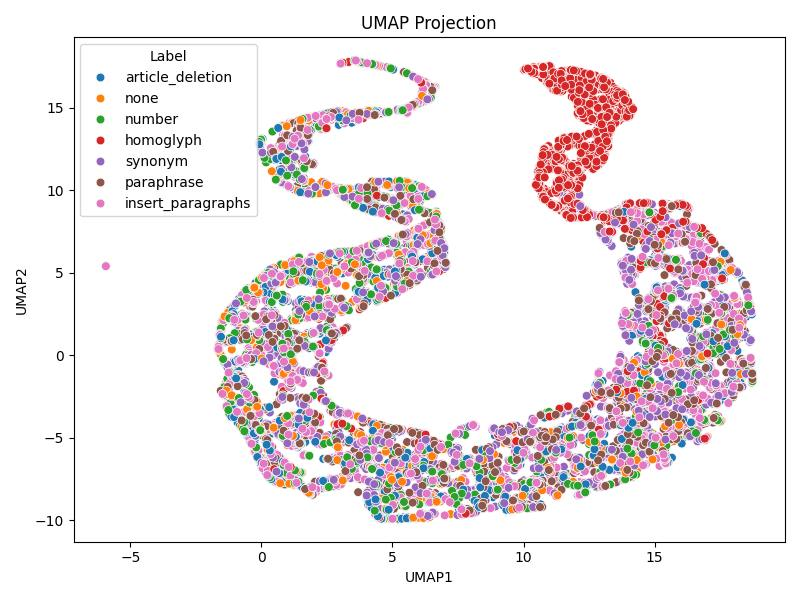
\includegraphics[width=1\linewidth]{umap.jpg}
  \caption{
    UMAP-projection of texts from RAID categorized by attack types.   }
  \label{fig:umap}
\end{figure}

The statistical metrics presented in Table 4 (pertaining to the first subset of the M4GT dataset) reveal significant variations in U) across different class labels. This observed variability in UE values provides a discriminative feature space that enables effective separation between text samples originating from different generative sources.

\begin{table}[ht]
\centering
\begin{tabular}{llrrrrr}
\toprule
\textbf{Metric} & \textbf{Label} & \textbf{Mean} & \textbf{Median} & \textbf{Std}  \\
\midrule
mean entropy   & Human   & 0.0038   & 0.0038   & 0.0006    \\
mean entropy   & Machine   & 0.0034   & 0.0033   & 0.0007   \\
perplexity    & Human   & 2.2668   & 2.2414   & 0.2887   \\
perplexity    & Machine   & 2.1129   & 2.0516   & 0.3197  \\
mc entropy    & Human   & 232.603  & 224.375  & 54.179   \\
mc entropy    & Machine   & 175.064  & 165.625  & 66.8385  \\
mahalanobis   & Human   & 125.960  & 124.123  & 23.165  \\
mahalanobis   & Machine   & 149.813  & 143.992  & 29.6482   \\
\bottomrule
\end{tabular}
\caption{Metrics for human and machine-generated texts}
\label{tab:metric-by-label}
\end{table}

\end{document}